\section{Namespaces as Document Clusters} \label{sec:namespaces-top}


In this chapter we discuss how the process of namespace discovery
can be automated.

First, in section~\ref{sec:namespaces} we describe identifier namespaces and
we compare the namespace discovery with cluster analysis techniques
applied to textual data and see how clustering algorithms can be
useful. Next, in section~\ref{sec:vsm}
we review the Vector Space Model (VSM): the traditional way of
representing a collection of documents as vectors, and then in
section~\ref{sec:ism} we introduce the Identifier VSM - which
is a way to represent identifier-definition relations in the
vector space. Finally we go over common similarity and distance
functions that are useful for document clustering in
section~\ref{sec:similarity-distance} and discuss how similarity
search can be made faster by using inverted index~\ref{sec:index}.



\subsection{Namespaces in Mathematical Notation} \label{sec:namespaces}

\textbf{TODO:} rewrite a bit to keep the introduction in mind. Also refer to introduction

An \emph{identifier namespace} is a coherent structure where
each identifier is used only once and has a unique definition.

How to find a namespace? Namespaces can be constructed by
manually labeling each identifier/definition pair with appropriate
name. But this is very time consuming, and in this work we suggest
a different approach: use Machine Learning techniques for
discovering namespaces automatically from a collection of scientific
documents containing mathematical formulae.


Many modern programming languages use namespaces for modularity.
For example, in the Java programming language \cite{gosling2014java}
namespaces are called ``packages'' and
a class may refer to classes from other packages via the \texttt{import}
statement.

% Example?


Typically in a well-designed application, we can distinguish between
two types of application packages \cite{evans2004domain}:

\begin{itemize}
  \item \emph{type 1}: domain-specific packages that deal with one particular concept, and
  \item \emph{type 2}: packages that use many other packages of the first type
\end{itemize}


For example, we have an application \verb|org.company.app|
with several domain-specific packages: \verb|org.company.app.domain.user|
with classes related to users, \verb|org.company.app.domain.account|
with classes related to user accounts, and a system-related package
\verb|org.company.app.tools.auth| that deals with authentication and
authorization. Then we also have a package \verb|org.company.app.web.manage|,
which belongs to the type 2: it handles web requests
while relying on classes from \verb|user| and \verb|account| to
implement the business logic and on \verb|auth| for making sure the
requests are authorized.

We can observe that the type 1 packages are mostly self-contained
and not highly coupled between each other,
but type2 packages mostly use other packages of type 1: they
depend on them.

\ \\

We can extend this idea to scientific documents and identifier
namespaces. A document can be seen as a class that uses concepts defined
in other documents. Then the documents can be grouped such that
some groups are of \emph{type 1}: they define the namespaces. In some
sense the documents of type 1 are ``pure'' - they contain infromation
about closely related concepts and not highly coupled
with other document groups. But some documents are of \emph{type 2} and they
are not pure: they draw from different concepts.


This intuition allows us to have the following assumptions:

\begin{enumerate}
 \item documents are ``mixtures'' of namespaces: they take identifiers from several namespaces
 \item there are some documents are more ``pure'' than others: they either take identifiers exclusively from one namespace or from few very related namespaces
\end{enumerate}


With these assumptions we can refer to ``pure'' groups as
\emph{namespace defining} groups. These groups can be seen as
``type 1'' packages: they define namespaces that are used by other
``type 2'' document groups.


Additionally, we can assume that there is a strong correlation
between identifiers in a document and the namespace of the document,
and this correlation can be exploit to categorize
documents into groups.


% The goal of this work is to automatically discover identifier namespaces in
% mathematical notation. But mathematical notation does not exist in isolation
% and it is usually used in documents. Therefore we can approximate
% namespace discovery from notation by namespace discovery from scientific
% documents.


Thus by combining these assumptions we can conclude that it should
be approximate the process of namespace discovery by discovering
groups of namespace defining documents, and this can be done by
applying cluster analysis techniques to documents, represented
by identifiers they contain.

In the next section we will argue why we can use traditional
document clustering techniques and what are the characteristics
that texts and identifiers have in common.


\subsection{Discovering Namespaces with Document Cluster Analysis} \label{sec:clusters-namespaces}


We believe that cluster analysis techniques developed for
text documents should work for identifiers.

Let us consider the characteristics of text data:

There are many distinct words in natural language. For example,
if $\mathcal V$ is a set of all possible words, then usually $|\mathcal V| \approx 10^5$,
but each individual document may contain only 500 distinct words, or
sometimes even less if we consider sentences or small documents
(e.g. tweets)

number of words across different document may wary a lot

 word distributions follow Power Laws (e.g. Zipf's law)


The identifiers have the same properties! 

\ \\


Natural languages suffer from lexical problems of variability and ambiguity,
and the two main problems are synonymy and polysemy \cite{deerwester1990indexing}
\cite{gliozzo2009semantic}:

\begin{itemize}
\itemsep1pt\parskip0pt\parsep0pt
  \item two words are \emph{synonymous} if they have the same meaning
        (for example, ``word'' and ``term'' are synonyms),
  \item a word is \emph{polysemous} is it can have multiple meanings
        (for example, ``trunk'' can refer to a part of elephant or a part of a car).
\end{itemize}


We can note that identifiers have the same problems. For example,
in Information Theory, the Shannon Entropy is usually denoted by
``$H$'', but sometimes it is also denoted by ``$I$'' or by ``$S$'',
thus these identifiers may be seen as synonyms.
Also, ``$E$'' can stand both for ``Energy'' and ``Expected value'',
so ``$E$'' is polysemous.

These problems have been studied in Information Retrieval and
Natural Language Processing literature.
One possible solution for the polysemy problem is Word Sense Disambiguation
\cite{jurafsky2000speech}: either replace a word with its sense
\cite{stokoe2003word} or append the sense to the word, for example
if the polysemous word is ``bank'' with meaning ``financial institution'',
then we replace it with ``bank\_finance''. The same idea can be used
for identifiers, for example ``$E$'' can be replaced with ``$E$\_energy''.
% We will expand this idea in the chapter~\ref{sec:ism}

Document clustering techniques usually use Vector Space Models
\cite{oikonomakou2005review} \cite{aggarwal2012survey} to represent documents.
We can define ``Identifier Spaces'' analogous to Vector Space Models.
We assume that Identifier Spaces exhibit the same characteristics as
traditional Vector Space Models, and thus

In the next section we review the Vector Space Model,
and then introduce the Identifier VSM in the chapter~\ref{sec:ism}

Then we can apply cluster analysis techniques to document-identifier matrices.


\subsection{Vector Space Model} \label{sec:vsm}

Vector Space Model is a statistical model for representing documents
in some (very high dimensional) vector space. It is an Information Retrieval
model \cite{manning2008introduction}, but it is also used for various
Text Mining tasks such as Document Classification \cite{sebastiani2002machine}
and Document Clustering \cite{oikonomakou2005review} \cite{aggarwal2012survey}.

The process of transforming a text to its vector representation is
called ``vectorization''. But before documents can be
vectorized they are preprocessed. The preprocessing usually consists of the
following steps:

\begin{itemize}
\itemsep1pt\parskip0pt\parsep0pt
  \item tokenization: extracting individual words from the text;
  \item stop words removal: removes functional words that have no discriminative power;
  \item word normalization (includes stemming or lemmatization): reduces words to some common form;
\end{itemize}

There are two assumptions made about the data:

\begin{itemize}
\itemsep1pt\parskip0pt\parsep0pt
  \item \emph{Bag of Words assumption}: the order of words is not important,
     only word counts;
  \item \emph{Independence assumption}: we treat all words as independent.
\end{itemize}

% Bag of Words = unordered list of terms
% good enough for topic similarity

Both assumptions are quite strong, but nonetheless this method often
gives good results.


Document-Term Matrix - representation of a document for text analysis
each row of the matrix - is a ''document vector''
each component of the document vectors is a concept, a key word, or a term, but usually it's terms
documents don't contain many distinct words, so the matrix is sparse


Notation:
let $\mathcal D = \{d_1, \ ... \ , d_n \}$ be a set of $m$ documents
and let $\mathcal V = \{t_1, \ ... \ , t_m \}$ be a set of $n$ terms (the vocabulary).
Each document is set of weighed terms $d_i = \{ w_1, \ ... \ , w_m \}$
where $w_j$ is the weight of term $t_j$.

There are following term weighting schemes \cite{manning2008introduction}:

\begin{itemize}
\itemsep1pt\parskip0pt\parsep0pt
  \item binary: 1 if a term is present, 0 otherwise
  \item term frequency (TF): number of occurrences of the term in a document
  \item document frequency (DF): number of documents containing the term
  \item TF-IDF: combination of TF and inverse DF
\end{itemize}


\textbf{Term Frequency (TF)} weights terms by local frequency in the document.
That is, the term is weighed by how many times it occurs in the document.
We can define TF formally as
$$\text{tf}(t, d) = \big| \{ t' \in d  \ : \ t' = t \} \big|$$


\textbf{Sublinear TF}: sometimes the term is used too often in
a document and we want to reduce its influence compared to
other less frequent tokens. This can be done by applying
some sublinear transformation to TF, for instance, a squared root
$\sqrt{\text{tf}(w, d)}$ or a logarithm $\log \text{tf}(w, d)$.


\textbf{Document Frequency (DF)} weights terms by their global frequency
in the collection, which is the number of documents that contain the token.
Formally it can be defined as
$$\text{df}(t, \mathcal D) = \big| \{ d \in \mathcal D \ : \  t \in d \} \big|$$


\textbf{Inverse Document Frequency (IDF)}: more often we are interested
in domain specific words than in neutral words, and these domain specific
words tent to occur less frequently and they usually have more discriminative
power: that is, they are better in telling one document apart from another.
So IDF should give more weights to rare words rather than to frequent words.
Typically IDF is defined as follows:
$$\text{idf}(t, \mathcal D) = \log \cfrac{ |\mathcal D| }{\text{df}(t, \mathcal D)}$$
% also can be some Entropy-based measure


A good weighting system gives the best performance when it assigns 
more weights to terms with high TF, but low DF \cite{salton1988term}.
This can be achieved by combining both TF and IDF
schemes. TF is good for getting high frequency words, but using
just TF is not enough if high frequency words are contained in
many documents, thus need a collection dependent factor that favors
terms that are contained in fewer documents: IDF.

Usually a sublinear TF is used to avoid the dominating effect of
words that occur too frequently. As the result, terms appearing
too rarely or too frequently are ranked low.

So, we can combine TF and IDF then my multiplying:
$$\text{tf-idf}(t, d \mid \mathcal D) = (1 + \log \text{tf}(t, d)) \cdot \log \cfrac{|\mathcal D|}{\text{df}(t, \mathcal D)}$$


\ \\

Once the weighting scheme is established, documents can be represented
by vectors $d_i = (w_1, \ ... \ w_m)$ where $w_j$ is the weight of term
$t_j$.

Then these vectors can be put together to form a matrix. Let $D$ be
a $m \times n$ matrix, where rows of $D$ are indexed by terms $t_i$,
columns of $D$ are indexed by documents $d_j$, and element $(D)_{ij}$
is a weight $w_i$ of term $t_i$ in document $d_j$. Then
such matrix $D$ is called a \emph{term-document matrix}.

Alternatively, $D$ can be $n \times m$ matrix with rows being indexed
by documents $d_j$ and columns - by terms $t_i$. Then such $D$ is called
\emph{document-term matrix}. Note that if $D$ is a term-document matrix,
then $D^T$ is a document-term matrix. In Information Retrieval
literature term-document matrices are used more often, than
document-term matrices, but in some applications, like Clustering,
it is more convenient to use document-term matrix.


Let us consider the column space of the term-document matrix $D$.
The column of $D$ are documents from the corpus $\mathcal D$,
so the column space of $D$ contains document vectors where
dimensions are terms $t_1,  t_2, \ ... \ , t_m$. This vector space is
called \emph{Document VSM}


\begin{figure}[h]
\centering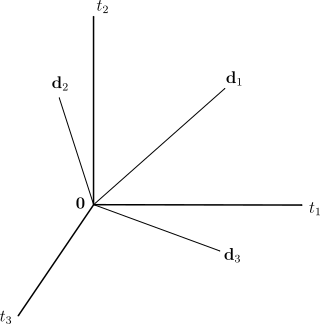
\includegraphics[width=0.6\textwidth]{document-vsm.png}
\caption{\textbf{TODO redraw in vector}}
\label{fig:document-vsm}
\end{figure}


Alternatively, we can consider the row space of $D$. This is
called the \emph{Term VSM}: the vectors in this space are terms
and they are indexed by documents $d_1, d_2,  \ ... \ , d_n$.


\begin{figure}[h]
\centering\includegraphics[width=0.6\textwidth]{term-vsm.png}
\caption{\textbf{TODO redraw in vector}}
\label{fig:term-vsm}
\end{figure}


%problems of VSMs:
%Text VSM can't deal with lexical ambiguity and variability
%e.g.: "he's affected by AIDS" and "HIV is a virus" don't have any
%words in common
%so in the TextVSM the similarity is 0: these vectors are orthogonal
%even though the concepts are related
%on the other hand, similarity between "the laptop has a virus"
%and "HIV is a virus" is not 0: due to the ambiguity of "virus"



\subsection{Identifier Space Model} \label{sec:ism}

The Vector Space Model gives a good foundation. In this work documents
are not represented by words they contain, but rather by identifiers they
have. Because  words and identifiers exhibit similar properties
(see section~\ref{sec:clusters-namespaces}) we can replace the
Term VSM by \emph{Identifier VSM}: a vector space where documents are represented as
vectors indexed by identifiers they contain.
Thus, the ``vocabulary'' of this space is $\text{id}_1, \ ... \ , \text{id}_k$, and
documents are represented as $d_j = (w_1, \ ... \ , w_k)$ where
$w_i$ is the weight of identifier $\text{id}_i$.

Then we can define an identifier-document matrix $D$ as $k \times n$
matrix where columns are documents and rows are identifers.

The Identifer VSM also suffers from the problems of polysemy
and synonymy (see section~\ref{sec:clusters-namespaces}). They
can be solved by extracting definitions for all the identifers
and incorporating these definitions into the Identifier VSM.

There are three ways of adding the definition information into
Identifier VSM:


\begin{itemize}
\itemsep1pt\parskip0pt\parsep0pt
  \item use only identifier information, and no not include the definitions;
  \item use ``weak'' identifier-definition association: include identifiers and
        definitions as separate dimensions;
  \item use ``strong'' association: append definition to identifier.
\end{itemize}

To illustrate how it is done, consider two relations ($\lambda$, ``regularization'')
and ($w$, ``weight vector'')


\begin{itemize}\itemsep1pt\parskip0pt\parsep0pt
  \item no definitions: dimension of the Identifier VSM are ($\lambda$, $w$)
  \item ``weak'' association:  dimensions are ($\lambda$, $w$, regularization, weight vector)
  \item ``strong'' association:  dimensions are ($\lambda$\_regularization, $w$\_weight vector)
\end{itemize}



\subsection{Similarity Measures and Distances} \label{sec:similarity-distance}

Once the documents are represented in some vector space, we need to
define how to compare these documents to each other. There are two
ways of doing this: using a similarity function that tells how similar
two objects are (the higher values, the more similar the objects),
or using a distance function, sometimes called ``dissimilarity function'',
which is the opposite of similarity (the higher the values, the less similar
the objects).

We will consider the following similarity and distance functions:


\begin{itemize}\itemsep1pt\parskip0pt\parsep0pt
  \item Euclidean distance
  \item Inner product (or dot product)
  \item Cosine similarity
  \item Jaccard coefficient
\end{itemize}


\subsubsection{Euclidean Distance} \ \\

The Euclidean distance function is the most commonly used distance
function in vector spaces. Euclidean distance corresponds to
the geometric distance between two data points in the vector space.
For example, if we have two points $\mathbf x$ and
$\mathbf z$, then the Euclidean distance is the
length of the line that connects these two points.
It is defined as
$$\| \mathbf x - \mathbf z \| = \sqrt{ (\mathbf x - \mathbf z)^T (\mathbf x - \mathbf z) } = \sqrt{\sum_i (x_i - z_i)^2}$$

This distance is also often called ``$L_2$ distance''.


Let us rewrite the expression for calculating the Euclidean distance:
$$\| \mathbf x - \mathbf z \|^2 = (\mathbf x - \mathbf z)^T (\mathbf x - \mathbf z) =
\mathbf x^T \mathbf x - 2 \mathbf x^T \mathbf z + \mathbf z^T \mathbf z =
\| \mathbf x \|^2 + \| \mathbf z \|^2 - 2 \mathbf x^T \mathbf z$$

A useful way to think about Euclidean distance for document spaces
is to consider all three elements of this distance: individual
lengths of both vectors and the inner product between them.

Consider two document vectors $\mathbf d_1$ and $\mathbf d_2$ with lengths
$l_1$ and $l_2$ respectively. If these two documents have
no terms in common, then the inner product term $\mathbf d_1^T \mathbf d_2$
between them is 0, and therefore the (squared) distance is
$\| \mathbf d_1 \|^2 + \| \mathbf d_2 \|^2 = l_1^2 + l_2^2$.
However if we consider two documents of the same lengths
$l_1$ and $l_2$ that share several terms in common,
their inner product, then their inner product is no longer 0,
and therefore these documents become closer. Thus, the more terms
the documents have in common, the closer they are.


While Euclidean distance is useful for low-dimensional data,
it does not always work very well in high dimensions, especially
with sparse vectors such as document vectors \cite{ertoz2003finding}.
The problem is usually caused by the individual length components of
the distance function: if two documents have no words in common,
but they are not long, they can have the same distance as two long
documents that have plenty of words in common.

Consider the following example (from \cite{ertoz2003finding}):
There are 4 data points $\mathbf d_1, \mathbf d_2, \mathbf d_3, \mathbf d_4$
in 10-dimensional space indexed by terms $A_1, \ ... \ , A_{10}$

\begin{center}
\begin{tabular}{|c|cccccccccc|}
  \hline
~ &  $A_1$ &   $A_2$ &   $A_3$ &  $A_4$ &  $A_5$ &  $A_6$ &  $A_7$ &  $A_8$ &  $A_9$ &  $A_{10}$ \\
  \hline
$\mathbf d_1$ &  3 &  0 &  0 &  0 &  0 &  0 &  0 &  0 &  0 &  0 \\
$\mathbf d_2$ &  0 &  0 &  0 &  0 &  0 &  0 &  0 &  0 &  0 &  4 \\
  \hline
$\mathbf d_3$ &  3 &  2 &  4 &  0 &  1 &  2 &  3 &  1 &  2 &  0 \\
$\mathbf d_4$ &  0 &  2 &  4 &  0 &  1 &  2 &  3 &  1 &  2 &  4 \\
  \hline
\end{tabular}
\end{center}

The distance between $\mathbf d_1$ and $\mathbf d_2$ is
$\| \mathbf d_1 - \mathbf d_2\| = 5$, and the distance between
$\mathbf d_3$ and $\mathbf d_4$ is also $\| \mathbf d_3 - \mathbf d_4\| = 5$.
But when we think of these data points as documents, intuitively
$\mathbf d_3$ and $\mathbf d_4$ should be closer because they
have 7 terms in common, whereas $\mathbf d_1$ and $\mathbf d_2$ have none.

Thus if the data is sparse it is better to use different measures
of distance/similarity, preferably ones that ignore dimensions
where both vector have 0 values.


\subsubsection{Inner product} \ \\

The Euclidean distance consists of three components: lengths and the inner product.
Since the lengths may cause some problems, it is possible to take only
the inner product part at treat it as a similarity function:
the more similar two vectors are, the larger is their inner product.

Geometrically the inner product between two vectors $\mathbf x$ and $\mathbf z$
is defined as
$$\mathbf x \cdot \mathbf z = \|\mathbf x \| \, \| \mathbf z \| \, \cos \theta$$
where $\theta$ is the angle between vectors $\mathbf x$ and $\mathbf z$ \cite{huges2013calculus}.
If the vectors are perpendicular, then $\cos \theta = 0$,
and the inner product is also $0$. The perpendicular vectors are called \emph{orthogonal}.

The geometric definition makes sense from the Law of Cosine point of view.
Consider two vectors $\mathbf x$ and $\mathbf z$, and let
$\mathbf y = \mathbf x - \mathbf z$.
Then the Law of Cosines states that
$$\| \mathbf y \|^2 = \| \mathbf x \|^2 + \| \mathbf z \|^2 - 2 \, \| \mathbf x \| \, \| \mathbf z\| \, \cos \theta$$
(see fig.~\ref{fig:law-cosines}).
By replacing $\| \mathbf x \| \, \| \mathbf z\| \, \cos \theta$ with
the inner product $\mathbf x \cdot \mathbf z$ and $\mathbf y$ with $\mathbf x - \mathbf z$
we get the Euclidean distance
$$\| \mathbf x - \mathbf z \|^2 = \| \mathbf x \|^2 + \| \mathbf z \|^2 - 2 \, \mathbf x \cdot \mathbf z \, \cos \theta$$


\begin{figure}[h]
\centering\includegraphics[width=0.4\textwidth]{cosine-theorem.png}
\caption{\textbf{TODO redraw in vector} The Law of Cosine:
$\| \mathbf y \|^2 = \| \mathbf x \|^2 + \| \mathbf z \|^2 - 2 \, \| \mathbf x \| \, \| \mathbf z\| \, \cos \theta$}
\label{fig:law-cosines}
\end{figure}


In Linear Algebra, however, the inner product (also called ``Dot product'')
is defined differently as a sum of element-wise products of two vectors:
given two vectors $\mathbf x$ and $\mathbf z$, the inner product is
$\mathbf x^T \mathbf z = \sum_{i = 1}^n x_i \, z_i$ where $x_i$ and $z_i$
are $i$th elements of $\mathbf x$ and $\mathbf z$, respectively.
The geometric and algebraic definitions are equivalent \cite{huges2013calculus}.


Thus, for two documents $\mathbf d_1$ and $\mathbf d_2$, the more terms
these documents have in common, the bigger their dot product is, and
the more similar they are.

However the magnitude of each individual vector still matters. If one
document vector is particularly long compared to other vectors and it is not
orthogonal to them (i.e. $\cos \theta \ne 0$), then it is likely to be
one of the most similar vectors to others -- only because of its length.


\subsubsection{Cosine Similarity} \ \\

The important drawback of the Inner product is that it is very sensitive to
lengths of the vectors. Therefore it may make sense to consider only the angle
between them: the angle does not depend on the magnitude, but still
acts as a very good indicator of vectors being similar or not.

The angle between two vectors can be calculated from the geometric
definition of inner product. Recall that given
two vectors $\mathbf x$ and $\mathbf z$, the inner product is defined as
$\mathbf x \cdot \mathbf z = \|\mathbf x \| \, \| \mathbf z \| \, \cos \theta$.
By rearranging the terms we get
$$\cos \theta = \frac{\mathbf x \cdot \mathbf z}{\|\mathbf x \| \, \| \mathbf z \|}$$
and thus
$$\theta = \arccos \frac{\mathbf x \cdot \mathbf z}{\|\mathbf x \| \, \| \mathbf z \|}$$

Note, however, that it is not necessary to invert the cosine: the angle $\theta$
between two vectors ranges from $0$ to $\pi$, and cosine is monotonically
decreasing on this interval. Thus, $\cos \theta \in [-1, 1]$, and the smaller
the angle between two vectors, the bigger the cosine of this angle.
Document vectors typically do not have negative components (all weights are
positive), and thus, the angle between two vectors can be at most $\pi$,
and therefore $\cos \theta \in [0, 1]$.

Using this, we define \emph{cosine similarity} between two documents $\mathbf d_1$ and
$\mathbf d_2$ as
$$\text{cosine}(\mathbf d_1, \mathbf d_2) = \cfrac{\mathbf d_1 \cdot \mathbf d_2}{\|\mathbf d_1 \| \, \| \mathbf d_2 \|}$$

If the documents have unit lengths, then cosine similarity is the same as
dot product: $$\text{cosine}(\mathbf d_1, \mathbf d_2) = \cfrac{\mathbf d_1 \cdot \mathbf d_2}{\|\mathbf d_1 \| \, \| \mathbf d_2 \|} = \mathbf d_1 \cdot \mathbf d_2$$.
Thus we can unit-normalize all document vectors
(i.e. compute $\mathbf d' = \mathbf d / \| \mathbf d \|$ for all
$\mathbf d \in \mathcal D$) and then simply use the dot product to compute
similarity between two documents. This normalization is often
called ``cosine normalization'' in Information Retrieval.


Cosine similarity gives the similarity score between two document vectors.
What if instead we need a distance function? The maximal possible cosine
is 1 for two identical documents. Therefore we can define \emph{cosine distance}
between two vectors $\mathbf d_1$ and $\mathbf d_2$ as
$$d_c(\mathbf d_1, \mathbf d_2) = 1 - \text{cosine}(\mathbf d_1, \mathbf d_2)$$
The cosine distance is not a proper metric \cite{korenius2007principal},
but it is nonetheless useful.

Finally, there is a connection between the cosine distance and the Euclidean
distance \cite{korenius2007principal}.
Consider two unit-normalized vectors $\mathbf d_1' = \mathbf d_1 / \| \mathbf d_1 \|$ and
$\mathbf d_2' = \mathbf d_1 / \| \mathbf d_1 \|$.
The Euclidean distance between them is
$$\| \mathbf d_1' - \mathbf d_2' \|^2 = \| \mathbf d_1' \|^2 - 2 \, \mathbf d_1'^T \mathbf d_2' + \| \mathbf d_2 \|^2 = 2 - 2 \, \mathbf d_1'^T \mathbf d_2$$

Since the vectors are unit-normalized, we know that
$\text{cosine}(\mathbf d_1', \mathbf d_2') = \mathbf d_1'^T \mathbf d_2'$, so we have
$$\| \mathbf d_1' - \mathbf d_2' \|^2 = 2 \, \big(1 - \text{cosine}(d_1', d_2')\big) = 2 \, d_c(d_1', d_2')$$.


Thus we can use Euclidean distance on unit-normalized vectors
and interpret it as Cosine distance.


\subsubsection{Jaccard Coefficient} \ \\

\textbf{Jaccard similarity, jaccard distance}


\subsubsection{Other Similarity Measures} \ \\


Other commonly used similarity measures include:

\begin{itemize}
  \item Dice Coefficient: $\cfrac{d_1^T d_2}{\|d_1\|^2 + \| d_2\|^2}$
  \item Pearson correlation coefficient
  \item etc
\end{itemize}


\subsection{Inverted Index} \label{sec:index}

In databases, indexing techniques are used to make queries faster and
avoid full table scan. Inverted Index is an Information Retrieval technique
for achieving better retrieval speed by reducing the number of documents that
the system needs to examine \cite{manning2008introduction}.
This technique is also
useful for other Text Mining tasks such as computing document-document
similarity matrix, where each document is compared to every other document
in the document collection.

% describe what inverted index is
%


The main idea is to use the fact that documents usually contain only
a small portion of terms. For example, a number of distinct terms in
the corpus may be $10^5$, but typically individual documents do not
contain more than $500$ distinct terms. % cite?
Thus, when these documents have very sparse document vectors, and many
similarity functions used for documents ignore zero entries
(e.g. cosine similarity or Jaccard coefficient).

For the cosine to be non-zero, two documents need to share at least one term.
Therefore to find documents similar to document $d$, we use the index to
restrict the list of documents to compare to those that
have at least one term in common.

\textbf{TODO: }Describe the algorithm of building the index and using it for the 
similarity search \ref{algo:inverted-index}.

\begin{algorithm}
\caption{Inverted Index for similarity computations}
\label{algo:inverted-index}
\begin{algorithmic}[0]
  \Statex
  \Function{Build-Index}{documents $\mathcal D$}
    \Let{$V$}{all distinct terms from $\mathcal D$}
    \For{each $w_i \in V$}
      \Let{index$[w_i]$}{$\varnothing$}
    \EndFor
    \For{each $d \in \mathcal D$}
      \For{each $w_i \in d$}
        \Let{index$[w_i]$}{index$[w_i] \cup \{ \, d \, \}$}
      \EndFor
    \EndFor
    \State \Return{index}
  \EndFunction
\end{algorithmic}

\begin{algorithmic}[0]
  \Statex
  \Function{Return-Candidates}{document $d$, index}
    \For{each $w_i \in d$}
      \Let{$D_i$}{index$[w_i] - d$} \Comment{all documents containing $w_i$ except $d$}
    \EndFor
    \State \Return{$\bigcup_i D_i$}
  \EndFunction
\end{algorithmic}
\end{algorithm}


In the next section we will review some algorithms for document clustering,
and Inverted Index can be used to speed up similarity computations
needed for these clustering algorithms. 